% !TeX spellcheck = en_US
\section{Criminal law}
\subsection{Basics - ART 1 SCC}
\begin{compactitem}
	\item No penalty without a law.
	\item No one may be punished for an act unless it has been expressly declared to be an offense by the law.
	\item Legal principle requiring that one cannot be punished for doing something	that is not prohibited by law.
	\item \textbf{No retrospective} impact of newly enacted criminal sanctions.
\end{compactitem}

\subsection{Purpose of the criminal law}
The purpose of criminal law is to steer human actions and to discourage missteps through:
\begin{compactitem}
	\item threat of punishment (general prevention),
	\item to punish the perpetrator (special prevention) and
	\item to return the perpetrator to the correct path (re-integration into society).
\end{compactitem}

\subsection{Elements of crime}
\begin{compactenum}
	\item \textbf{Conduct (act or omission)}
	\item \textbf{Offense as describe din law}
	\item \textbf{Illegal, no justification} \\
		Justifications:
		\begin{compactitem}
			\item Act is required or permitted by the law (SCC 14)
			\item Legitimate self-defence (SCC 15)
			\item Legitimate act in a situation of necessity (SCC 17)
			\item Consent of the victim
		\end{compactitem}
	\item \textbf{Culpable}\\
		a person is only liable to prosecution if he commits it willfully (SCC 12):
		\begin{compactitem}
			\item Intention
			\item Negligence (Fahrlässigkeit)
		\end{compactitem}
\end{compactenum}

\subsection{Criminal sanctions}
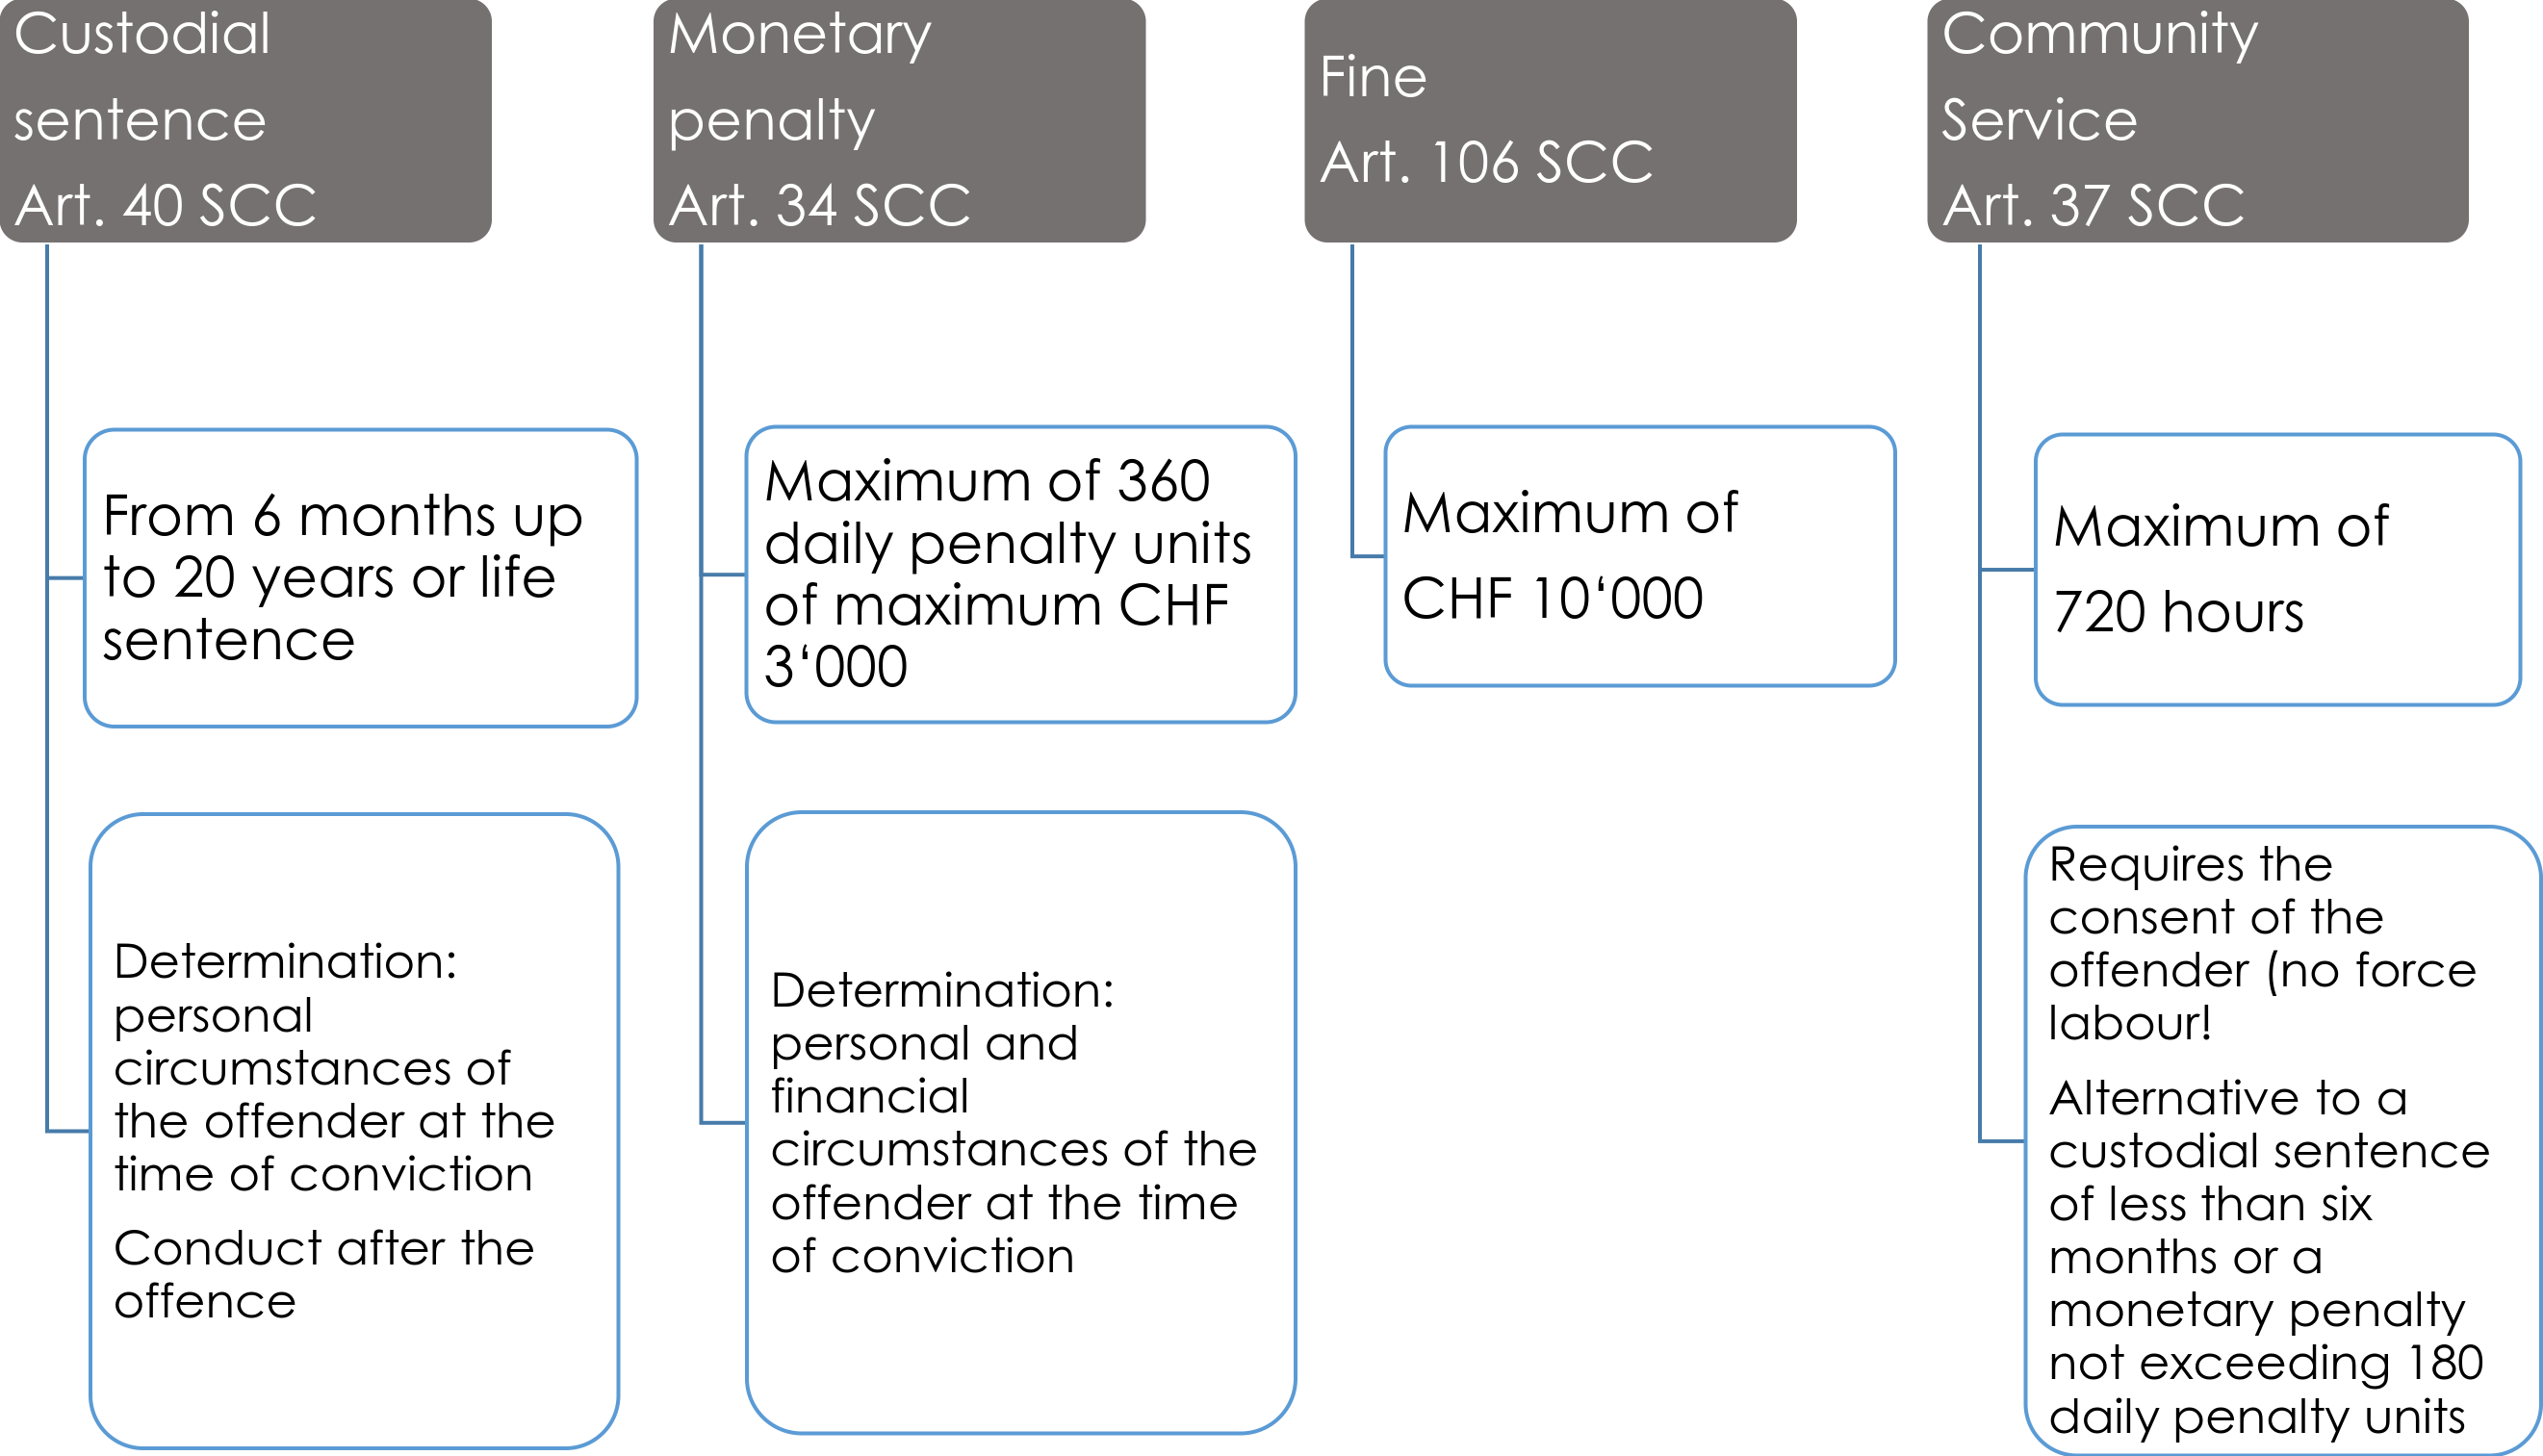
\includegraphics[width=1\linewidth]{images/criminalsanctions}
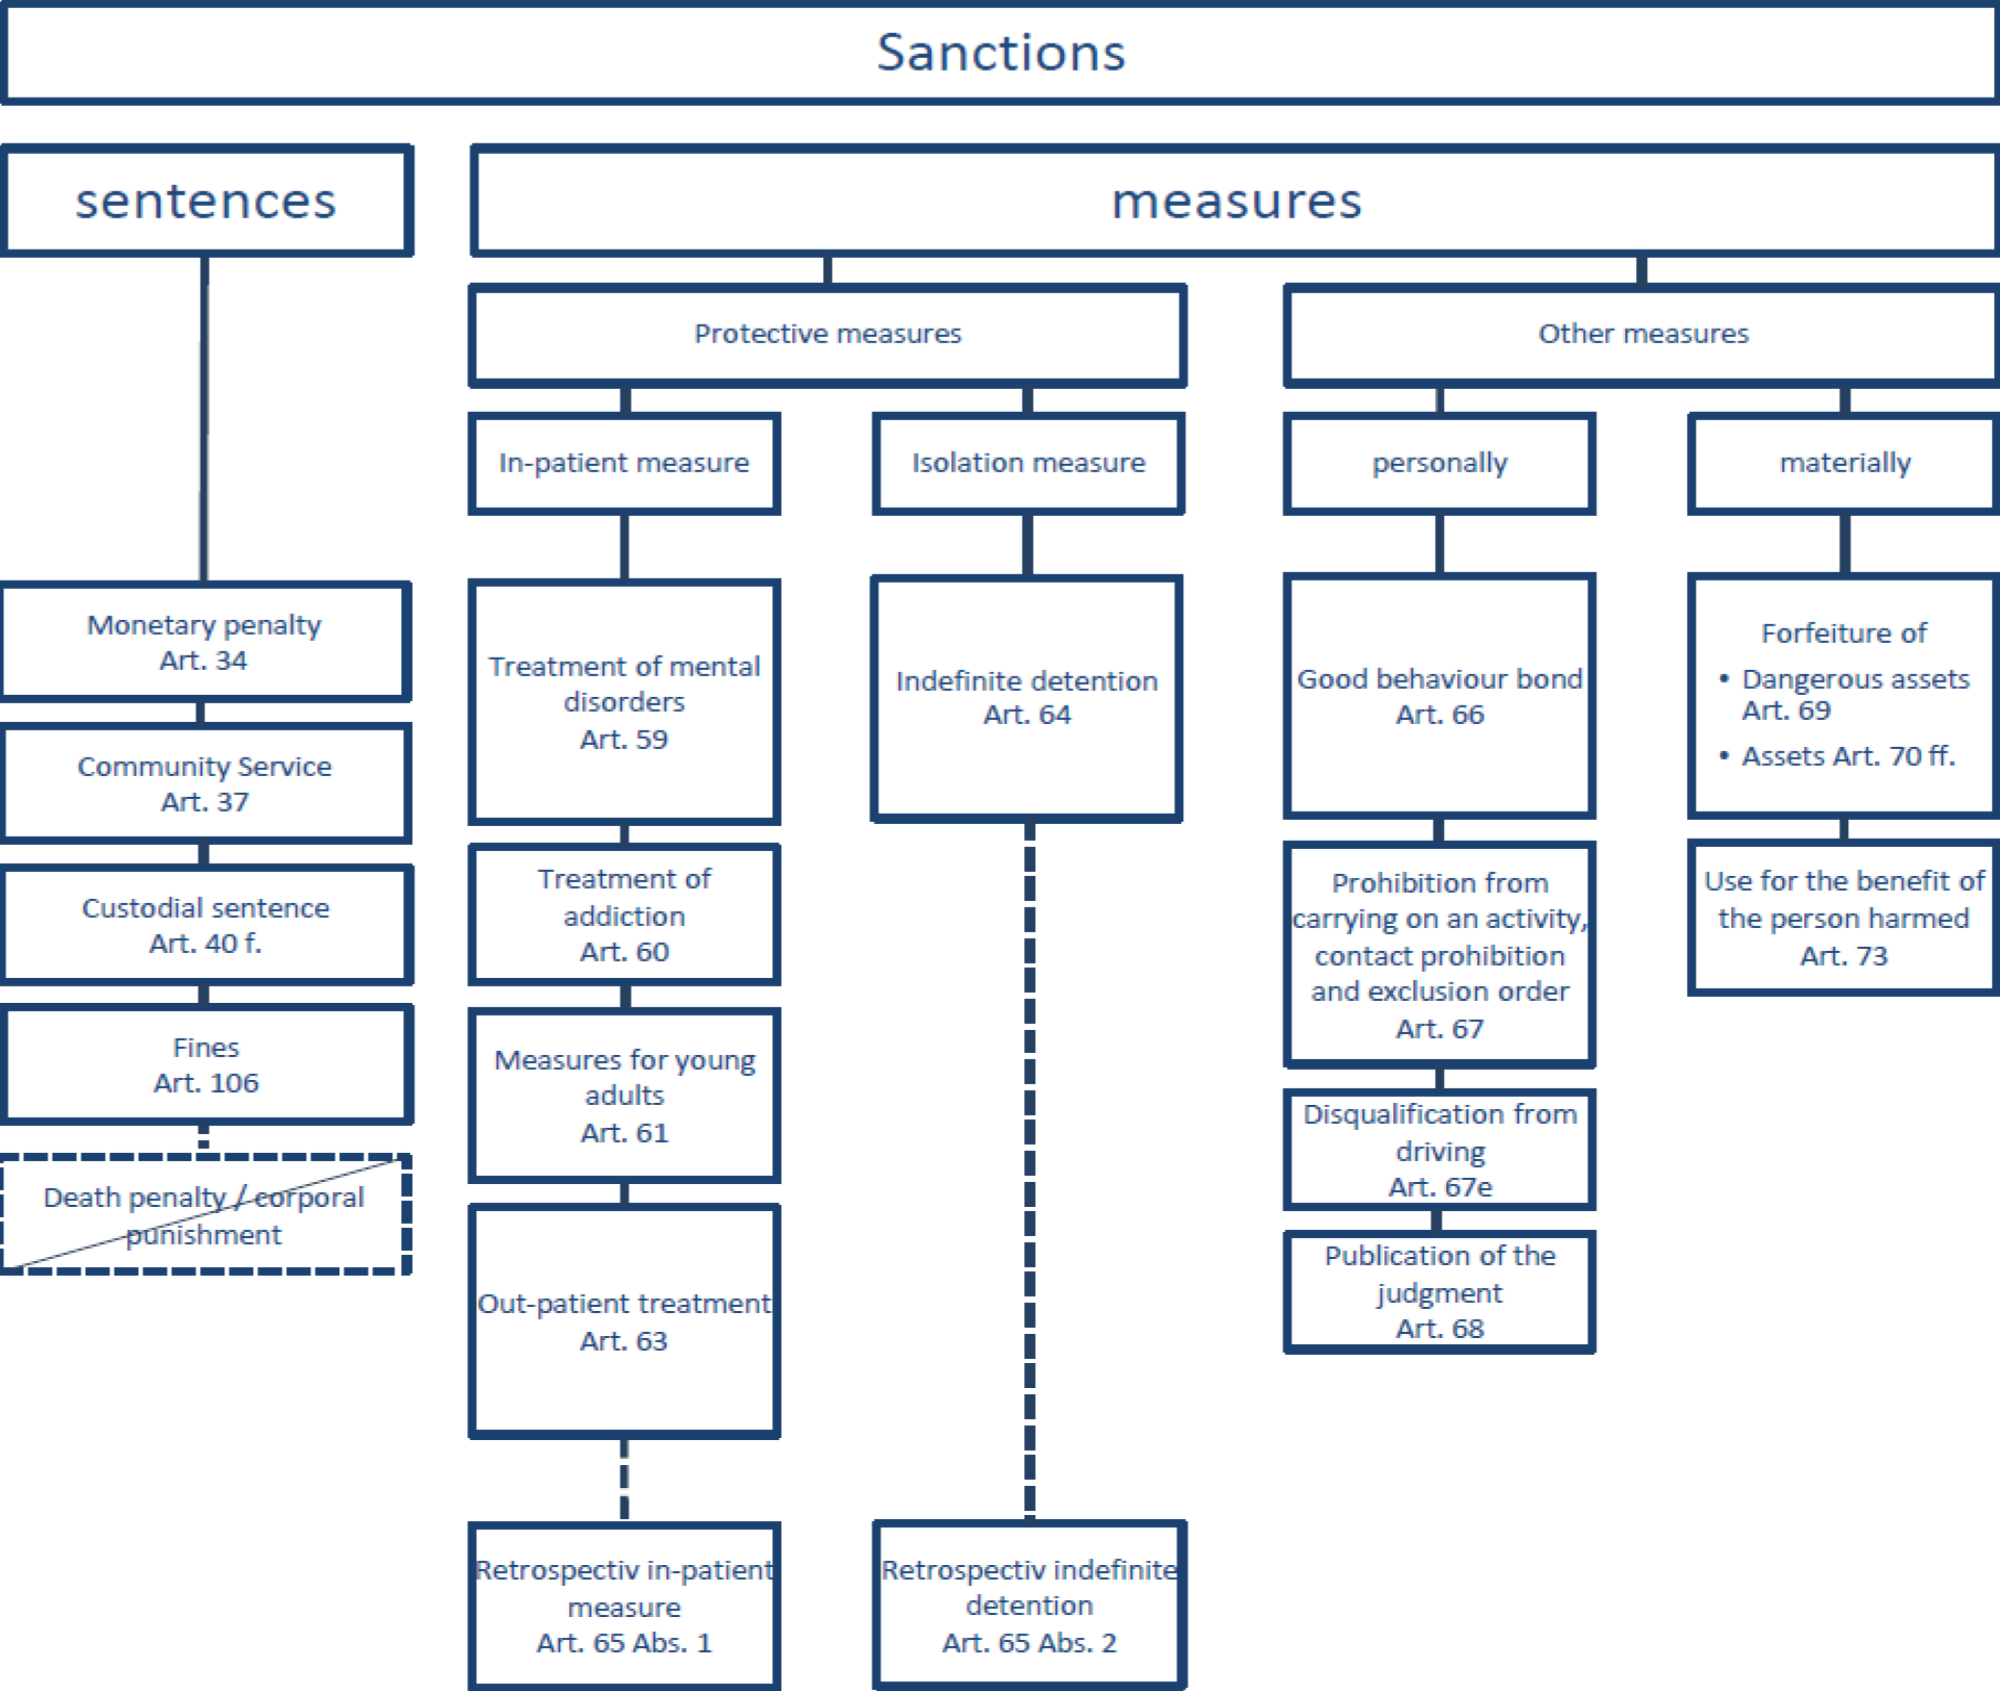
\includegraphics[width=1\linewidth]{images/criminalsanctions2}

\subsection{Criminal liability}
\textbf{Ex officio offense:}\\
Prosecution authorities prosecute the crime irrespective of a criminal complaint of the victim.\\
\textbf{Offenses prosecuted only based upon a criminal complaint (Art. 30 SCC):}\\
If an act is liable to prosecution only if a complaint is filed, any person who suffers harm due to the act may request that the person responsible be prosecuted. Time limit: The right to file a complaint expires after 3 months after the victim discovers the identity of suspect.

\subsection{Overview Offenses}
\begin{compactitem}
	\item Offences against Life and Limb
	\begin{compactitem}
		\item Intentional homicide (Art. 111), Murder (Art. 112), Manslaughter (Art. 113), Assault (Art. 122)
	\end{compactitem}
	\item Offences against Property
	\begin{compactitem}
		\item Misappropriation (Art. 138), Theft (Art. 139, Robbery (Art. 140), Unlawful use of financial assets (Art. 141bis), Unauthorised obtaining of data (Art. 143), Unauthorised access to a data processing system (Art. 143bis), Damage, (Art. 144), Damage to data (Art. 144bis), Misappropriation (Art. 145), Fraud (Art. 146), Computer fraud (Art. 147)
	\end{compactitem}
	\item Offences against Personal Honour and in Breach of Secrecy or Privacy (Art. 173 SCC ff)
	\begin{compactitem}
		\item Defamation (Art. 173), Insult (Art. 177), Breach of the privacy of a sealed document (Art. 179), Listening in on and recording the conversations of others (Art. 179bis), Unauthorised recording of conversations (Art. 179ter), Breach of secrecy or privacy through the use of an image carrying, device (Art. 179quater)
	\end{compactitem}
	\item Felonies and Misdemeanours against Liberty
	\item Offences against Sexual Integrity
	\item Felonies and Misdemeanours constituting a Public Danger and against Public Health
	\item ...
\end{compactitem}

\subsection{Computer crimes}
\textbf{Computer Crimes in the strict sense:}
\begin{compactitem}
	\item Unauthorized obtaining of data Art. 143
	\item Unauthorized access to a data processing system Art. 143bis (hacking)
	\item Damage to data Art. 144bis
	\item Computer fraud Art. 147
	\item Obtaining a service without payment Art. 150
	\item Production and marketing of equipment for the unauthorized, decoding of encoded services Art. 150bis
	\item Obtaining personal data without authorization Art. 179novies
	\item Forgery (Nachahmung, Urkundenfälschung) Art. 251-254 StGB / Art. 110 Abs. 4 + 5
\end{compactitem}
\textbf{Crimes committed by use of computers:}
\begin{compactitem}
	\item Representations of acts of violence Art. 135
	\item Offenses against Personal Honor and in Breach of Secrecy or Privacy Art. 173-178
	\item Pornography, Art. 197 StGB
	\item Racial discrimination Art. 261bis
	\item Misuse of a cheque card or credit card (Art. 148)
\end{compactitem}

\subsection{Definition personal data}
Personal data is all information relating to an identified or identifiable person. Sensitive personal data is data on:
\begin{compactitem}
	\item religious, ideological, political or trade union-related views or activities,
	\item health, the intimate sphere or the racial origin,
	\item social security measures,
	\item administrative or criminal proceedings and sanctions.
\end{compactitem}

\subsection{Rights of data subjects}
\begin{compactitem}
	\item Right to be informed
	\item Right of access
	\item Right to rectification
	\item Right to object to processing
	\item Right to restrict processing
	\item The right to erasure: no “right to be forgotten” as such
\end{compactitem}

\subsection{Data and Information provided / collected when using online services}
\begin{compactitem}
	\item Data provided by the data subject at the time of registration:\\
		Name, e-mail address, telephone number, date of birth, home address, mother tongue, gender -> personal data!
	\item Data collected while an online service is used\\
		IP-address -> personal data!\\
		device model, serial number, location, ISP?\\
		online status, interaction and use pattern use behavior?
	\item Data collected when purchases are made:\\
		credit card information, identification information, home address
\end{compactitem}

\subsection{Criminal provision under copyright law}
\begin{compactitem}
	\item Infringement of related rights, i.e. rights of performers, labels, broadcasters (Art. 69 Copyright Act)
	\item Criminal proceedings are initiated on \textbf{complaint}, sanction is \textbf{1 year or a monetary penalty}
	\item \textbf{Prosecution ex officio} if infringements were committed for commercial gain; sanction is up to \textbf{5 years or monetary penalty}
\end{compactitem}
If you do not have a license from the author/right holder to do so, the following is deemed a criminal offense:
\begin{compactitem}
	\item use a work under a false designation;
	\item publish a work;
	\item modify a work, create a derivative work;
	\item produce copies of a work in any manner;
	\item offer, transfer or otherwise distribute copies of a work;
	\item perform or present a work or makes a work perceptible somewhere else either directly or with the help of any kind of medium;
	\item make a work available through any kind of medium, including broadcasting, in such a way that persons may access it from a place and at a time individually chosen by them; (online!)
	\item rent out a computer program.
\end{compactitem}

\subsection{Criminal provision under trademark law}
\begin{compactitem}
	\item Infringement of a trade mark right (Art. 61 Trademark Act)
	\item Fraudulent use of trade marks (Art. 62 Trademark Act)
	\item Use of a guarantee or collective mark contrary to the regulations (Art. 63 Trademark Act)
	\item Use of incorrect indications of source (swissness from China!) (Art. 64 Trademark Act)
	\item Criminal proceedings are initiated on \textbf{complaint}, sanction is \textbf{1 year or a	monetary penalty}
	\item \textbf{Prosecution ex officio} if infringements were committed for commercial gain; sanction is up to \textbf{5 years or monetary penalty}
\end{compactitem}
Infringement of a trade mark right (Art. 61 Trademark Act) (Verstoss):
\begin{compactitem}
	\item \textbf{appropriate, counterfeit or imitate} the trade mark of the other person;
	\item place goods on the market or provide services, or offer, import, export, or advertise such goods or services under the appropriated, counterfeited or imitated trade mark.
\end{compactitem}
Fraudulent use of trade marks (Art. 62 Trademark Act) (Betrügerisch):
\begin{compactitem}
	\item unlawfully label goods or services with the trade mark of another person in order to \textbf{mislead} and thereby give the impression that the goods or services are original goods or services;
	\item offer or places goods or services on the market \textbf{as original} goods or services, or offers or provides original services that unlawfully bear the trade mark of another.
\end{compactitem}

\subsection{Legal base}
\subsubsection{Corporate criminal liability - ART. 102 SCC}
If a felony or misdemeanor is \textbf{committed in an undertaking in the exercise of commercial activities} in accordance with the objectives of the undertaking and if it is not possible to attribute this act to any specific natural person \textbf{due to the inadequate organization of the undertaking}, then the felony or misdemeanor is attributed to the undertaking. In such cases, the undertaking is liable to a \textbf{fine} not exceeding 5 million francs.\\
A company is penalized for \textbf{money laundering and bribery} (active/passive) irrespective of the criminal liability of any natural persons, provided the \textbf{undertaking has failed to take all the reasonable organizational measures} that are required in order to prevent such an offense.

\subsubsection{Intent - Negligence - ART. 12 SCC}
A person commits a felony or misdemeanor \textbf{willfully} if he carries out the act in the \textbf{knowledge} of what he is doing and in accordance with his \textbf{will}. A person acts willfully as soon as he regards the realization of the act as being \textbf{possible} and \textbf{accepts} this. A person commits a felony or misdemeanor through \textbf{negligence} if he \textbf{fails to consider or disregards the consequences} of his conduct due to a \textbf{culpable lack of care}. A lack of care is culpable if the person fails to exercise the care that is incumbent on him in the circumstances and commensurate with his personal capabilities.

\subsubsection{Felony – Misdemeanor - ART. 10 SCC}
\textbf{Felonies} are offences that result in a custodial sentence of \textbf{more than 3 years}. Examples: intentional homicide (Art. 111 SCC), murder (Art. 112 SCC), manslaughter (Art. 113 SCC). \\
\textbf{Misdemeanors} are offences that that result in a custodial sentence l\textbf{ess than 3 years or a monetary penalty}.

\subsubsection{Contravention - ART. 103 SCC}
\textbf{Contraventions} are acts that are punishable by a \textbf{fine}.

\subsubsection{Unauthorised obtaining of data - ART. 143 SCC}
\begin{compactenum}
	\item Any person who for his own or for another's \textbf{unlawful gain} obtains for himself or another \textbf{data} that is stored or transmitted electronically or in some similar manner and \textbf{which is not intended for him} and has been \textbf{specially secured to prevent his access} is liable to a custodial sentence not exceeding \textbf{five years or to a monetary penalty}.
	\item The unauthorized obtaining of data to the detriment of a relative or family member is prosecuted only on complaint.
\end{compactenum}

\subsubsection{Unauthorised access to a data processing system (hacking) - ART. 143bis SCC}
\begin{compactenum}
	\item Any person who \textbf{obtains unauthorized access} by means of data transmission equipment to a data processing system that has been \textbf{specially secured to prevent his access} is liable on complaint to a custodial sentence not exceeding \textbf{three years or to a monetary penalty}.
	\item Any person who markets or makes accessible passwords, programs or other data that he knows or must assume are intended to be used to commit an offense under paragraph 1 is liable to a custodial sentence not exceeding three years or to a monetary penalty.
\end{compactenum}

\subsubsection{Damage to data - ART. 144bis SCC}
\begin{compactenum}
	\item Any person who \textbf{without authorization} alters, deletes or renders unusable data that is stored or transmitted electronically or in some other similar way is liable on complaint to a custodial sentence not exceeding \textbf{three years or to a monetary penalty}. If the offender has caused \textbf{major damage}, a custodial sentence of from one to \textbf{five years} may be imposed. The offense is prosecuted ex officio.
	\item Any person who manufactures, imports, markets, advertises, offers or otherwise makes accessible programs that he knows or must assume will be used for the purposes described in paragraph 1 above, or provides instructions on the manufacture of such programs is liable to a custodial sentence not exceeding three years or to a monetary penalty. If the offender acts for \textbf{commercial gain}, a custodial sentence of from one to	\textbf{five years} may be imposed.
\end{compactenum}

\subsubsection{Computer fraud - ART. 147 SCC}
\begin{compactenum}
	\item Any person who with a view to his own or another's \textbf{unlawful gain}, by the \textbf{incorrect, incomplete or unauthorised use of data}, or in a similar way, influences the electronic or similar processing or transmission of data and as a result \textbf{causes the transfer of financial assets}, thus occasioning loss to another, or immediately thereafter conceals such a transfer is liable to a custodial sentence not exceeding \textbf{5 years or to a monetary penalty}.
	\item If the offender acts for \textbf{commercial gain}, he is liable to a custodial sentence not exceeding \textbf{10 years or to a monetary penalty of not less than 90 daily penalty units}.
	\item Computer fraud to the detriment of a relative or family member is prosecuted only on complaint.
\end{compactenum}

\subsubsection{Forgery of documents - ART. 251 SCC}
Any person who with the intent to cause financial loss or damage to another or in order to obtain an unlawful advantage for himself or another,
\begin{compactitem}
	\item produces a false document , falsifies a genuine document, uses the genuine signature or mark of another to produce a false document , falsely certifies or causes to be falsely certified a fact of legal significance or,
	\item makes use of a false or falsified document in order to deceive, is liable to a custodial sentence not exceeding \textbf{5 years} or to a monetary penalty.
\end{compactitem}

\subsubsection{Definition document - ART. 110 SCC}
Documents are written works intended and designed to \textbf{prove a fact of legal relevance}, or indications that are intended to prove such a fact.\textbf{ Recordings on image and data carriers} are equivalent to a written document, provided that they serve the same purpose. Includes also emails!

\subsubsection{Obtaining personal data without authorization - ART. 179novies SCC}
Any person who without authorization obtains from a data collection \textbf{personal data or personality profiles} that are particularly \textbf{sensitive} and that are \textbf{not freely accessible} is liable on complaint to a custodial sentence not exceeding \textbf{3 years or to a monetary penalty}.

\subsubsection{Criminal offence regarding processing of personal data - ART. 34 Federal Data Protection Act}
\textbf{Breach of obligations to provide information, to register or to cooperate}. On complaint, persons are liable to a \textbf{fine} if they:
\begin{compactitem}
	\item Breach their obligations in the context of a \textbf{request to access} by the data subject
	\item Fail to \textbf{notify the files of sensitive data} processed to the Data Protection Commissioner
	\item Provide the Commissioner with \textbf{false information} in the course of a case investigation or who \textbf{refuse to cooperate}
\end{compactitem}

\subsubsection{Criminal offense regarding processing of personal data - ART. 35 SCC}
\begin{compactenum}
	\item Anyone who \textbf{without authorization willfully discloses confidential, sensitive personal data or personality profiles that have come to their knowledge in the course oft heir professional activities} where such activities require the knowledge of such data is, on complaint, liable to a fine.
	\item The same penalties apply to anyone who without authorization willfully discloses confidential, sensitive personal data or personality profiles that have come to their knowledge \textbf{in the course of their activities for a person bound by professional confidentiality} or in the course of training with such a person.
	\item The unauthorized disclosure of confidential, sensitive personal data or personality profiles remains an offense \textbf{after termination} of such professional activities or training.
\end{compactenum}